\documentclass{article}
\usepackage{hyperref}
\usepackage{listings}
\usepackage{color}
\usepackage{xcolor}
\usepackage{geometry}
\usepackage{graphicx}
\usepackage{amsmath}
\usepackage{caption}
\usepackage{subcaption}
\usepackage[capitalise]{cleveref}
\usepackage{wrapfig}
\usepackage{amssymb}

\geometry{margin=1in}
\pdfminorversion=6

\newcommand\TODO[1]{\textcolor{red}{TODO: #1}}

\newcommand\header[2]{
    \begin{center}
        {\large
        UCSD CSE 167 Assignment #1: \\
        \vspace{0.3cm}
        \Large
        #2}
    \end{center}
}

\definecolor{dkgreen}{rgb}{0,0.6,0}
\definecolor{gray}{rgb}{0.5,0.5,0.5}
\definecolor{mauve}{rgb}{0.58,0,0.82}
\lstset{frame=tb,
        aboveskip=3mm,
        belowskip=3mm,
        showstringspaces=false,
        columns=flexible,
        basicstyle={\small\ttfamily},
        numbers=none,
        numberstyle=\tiny\color{gray},
        keywordstyle=\color{blue},
        commentstyle=\color{dkgreen},
        stringstyle=\color{mauve},
        breaklines=true,
        breakatwhitespace=true,
        tabsize=2
}

% Taken from https://tex.stackexchange.com/questions/83085/how-to-improve-listings-display-of-json-files

\colorlet{punct}{red!60!black}
\definecolor{delim}{RGB}{20,105,176}
\colorlet{numb}{magenta!60!black}

\lstdefinelanguage{json}{
    basicstyle=\normalfont\ttfamily,
    numberstyle=\scriptsize,
    stepnumber=1,
    numbersep=8pt,
    showstringspaces=false,
    breaklines=true,
    frame=lines,
    tabsize=2,
    literate=
     *{0}{{{\color{numb}0}}}{1}
      {1}{{{\color{numb}1}}}{1}
      {2}{{{\color{numb}2}}}{1}
      {3}{{{\color{numb}3}}}{1}
      {4}{{{\color{numb}4}}}{1}
      {5}{{{\color{numb}5}}}{1}
      {6}{{{\color{numb}6}}}{1}
      {7}{{{\color{numb}7}}}{1}
      {8}{{{\color{numb}8}}}{1}
      {9}{{{\color{numb}9}}}{1}
      {:}{{{\color{punct}{:}}}}{1}
      {,}{{{\color{punct}{,}}}}{1}
      {\{}{{{\color{delim}{\{}}}}{1}
      {\}}{{{\color{delim}{\}}}}}{1}
      {[}{{{\color{delim}{[}}}}{1}
      {]}{{{\color{delim}{]}}}}{1},
}

\hypersetup{colorlinks=true}


\begin{document}

\header{1}{3D Software Rendering}

The previous homework focused on 2D graphics (which is already quite important!). In this homework, we're going 3D. We will define shapes in 3D, project them onto the screen space, and render them. The projection is going to simulate how a camera (or our eyes) works: it 

\begin{figure}[h]
    \centering
    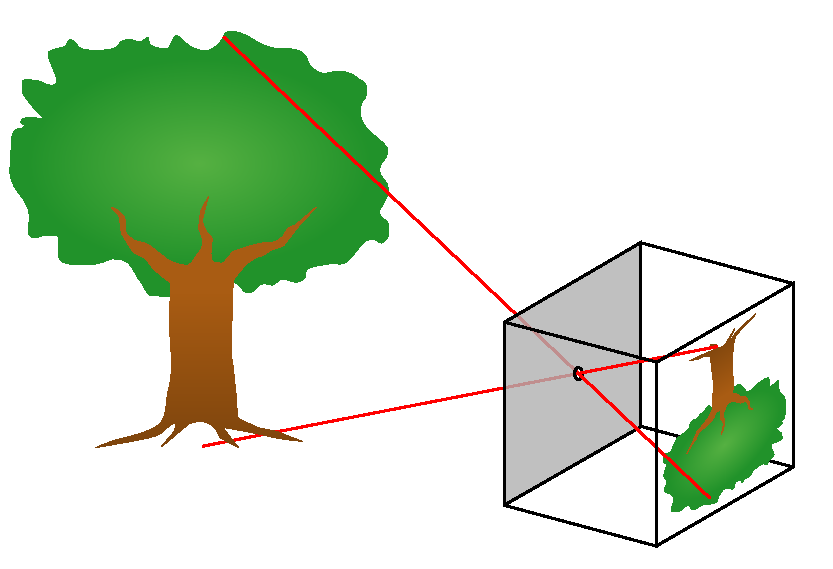
\includegraphics[width=0.5\linewidth]{imgs/pinhole.pdf}
    \caption{In this homework, we will implement 3D rendering by projecting 3D objects onto images. This is similar to a real-world camera. In particular, we will implement an ideal \href{https://en.wikipedia.org/wiki/Pinhole_camera}{pinhole camera}. Figure taken from \href{https://commons.wikimedia.org/wiki/File:Pinhole-camera.svg}{Wikipedia}.}
    \label{fig:pinhole}
\end{figure}

To facilitate the projection, we will focus on representing 3D surfaces, instead of the full volume. Instead of supporting multiple shapes (circles, squares, etc) like last time, we will focus on a single primitive: triangle. A main reason is that triangle has a very cool property: after perspective projection to 2D, it's still a triangle! (See \cref{fig:perspective}.) Many other shapes do not have this nice property -- a sphere projecting on to 2D can be an ellipse, a square projecting to the screen can become a general quadliteral.

\begin{figure}[h]
    \centering
    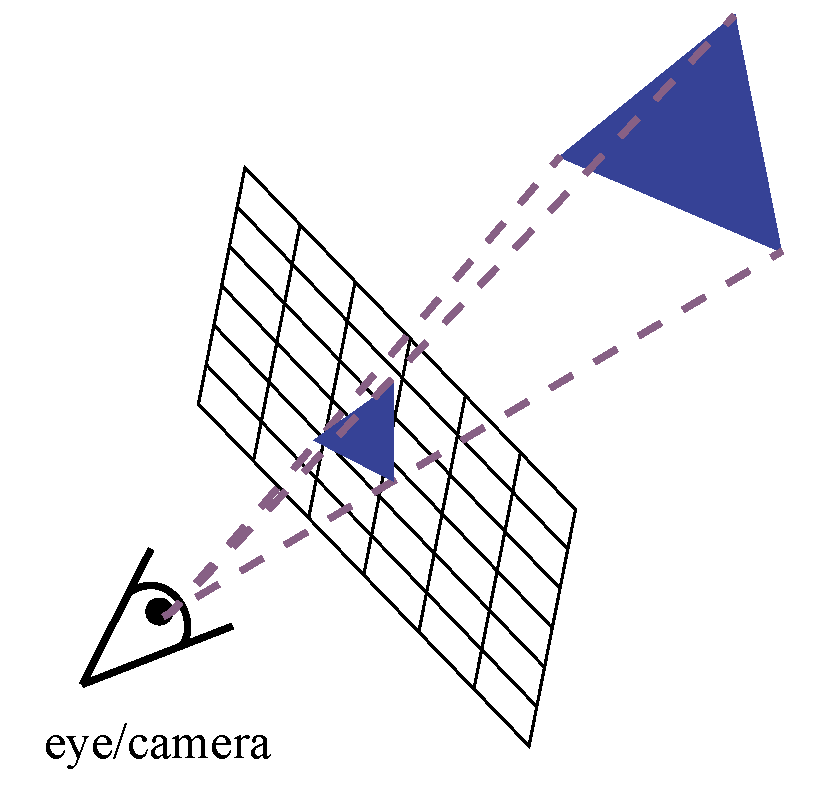
\includegraphics[width=0.5\linewidth]{imgs/perspective_projection.pdf}
    \caption{The perspective projection of a triangle.}
    \label{fig:perspective}
\end{figure}

\section{Rendering a single 3D triangle}
Let's start simple and render just a single 3D triangle. Our plan is to first project the triangle to a 2D image plane, then we can directly use the code from our previous homework to render the projected triangle.

\begin{figure}[h]
    \centering
    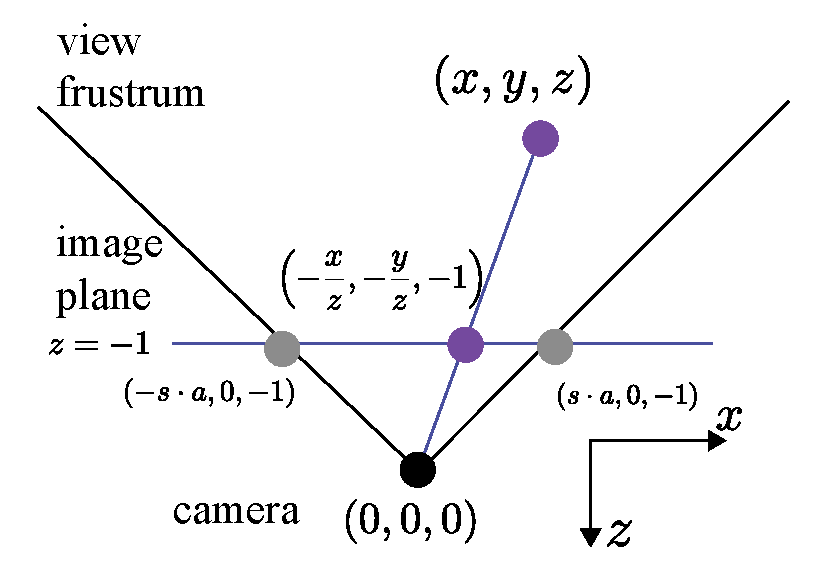
\includegraphics[width=0.5\linewidth]{imgs/perspective_transform.pdf}
    \caption{To perform perspective projection, we setup the coordinate system of the camera space so that the origin of the camera is at $(0, 0, 0)$, the camera is facing negative $z$-axis, $x$-axis is pointing right, and $y$-axis is pointing up. We put the image plane at $z=-1$. The perspective projection of a point $(x, y, z)$ is then simply finding the intersection between the line formed by the point and the camera origin with the image plane. Since our image plane has a finite extent, we further clips all point outside of $[-sa, -s, -1] \times [sa, s, -1]$ where $a$ is the aspect ratio ($\frac{\text{image width}}{\text{image height}}$) and $s$ is the scaling factor controlling the size of our image. The clipping defines a \emph{view frustrum}.}
    \label{fig:perspective_transform}
\end{figure}

How do we project the triangle then? It's significantly easier if we assume a particular coordinate system of our camera. We will lift this assumption in the later part of the homework (by, you guess it, applying 3D transformations). Let's assume in the \emph{camera space}, $x$-axis is pointing right, $y$-axis is pointing up, and $z$-axis is pointing away from the direction the camera is looking at (the $z$ is specified this way so that we are following a \href{https://en.wikipedia.org/wiki/Right-hand_rule}{right-handed} coordinate system). We also assume that the image plane is located at $z=-1$. \cref{fig:perspective_transform} shows that the perspective projection of a point $(x, y, z)$ boils down to computing the intersection between the line formed by the point and the camera origin with the image plane. The projected point $(x', y')$ is
\begin{equation}
\left(x', y'\right) = \left(-\frac{x}{z}, -\frac{y}{z}\right).
\label{eq:projection}
\end{equation}

Furthermore, we need to define the extent of the image plane (we can't have an image with infinite size!). Note that our image can be a rectangle (instead of a square). We define the extent of the image plane to be $[-sa, -s, -1] \times [sa, s, -1]$: $s$ is a scaling factor that controls the size of the image, and $a$ is the aspect ratio ($\frac{\text{image width}}{\text{image height}}$). As we will later show, $s$ is related to the \href{https://en.wikipedia.org/wiki/Field_of_view}{field of view} of a camera. Any point that lands outside of the extend of the image plane is discarded and not going to show up in our image. We call the set of points that are going to land on the image planes the \emph{view frustrum}. \cref{fig:perspective_transform} also visualizes the view frustrum.

Therefore, given a triangle with 3 vertices, we will project all three of them onto the image plane using \cref{eq:projection}. This generates a 2D triangle which we can then render using our previous homework's code.

\begin{figure}[h]
    \centering
    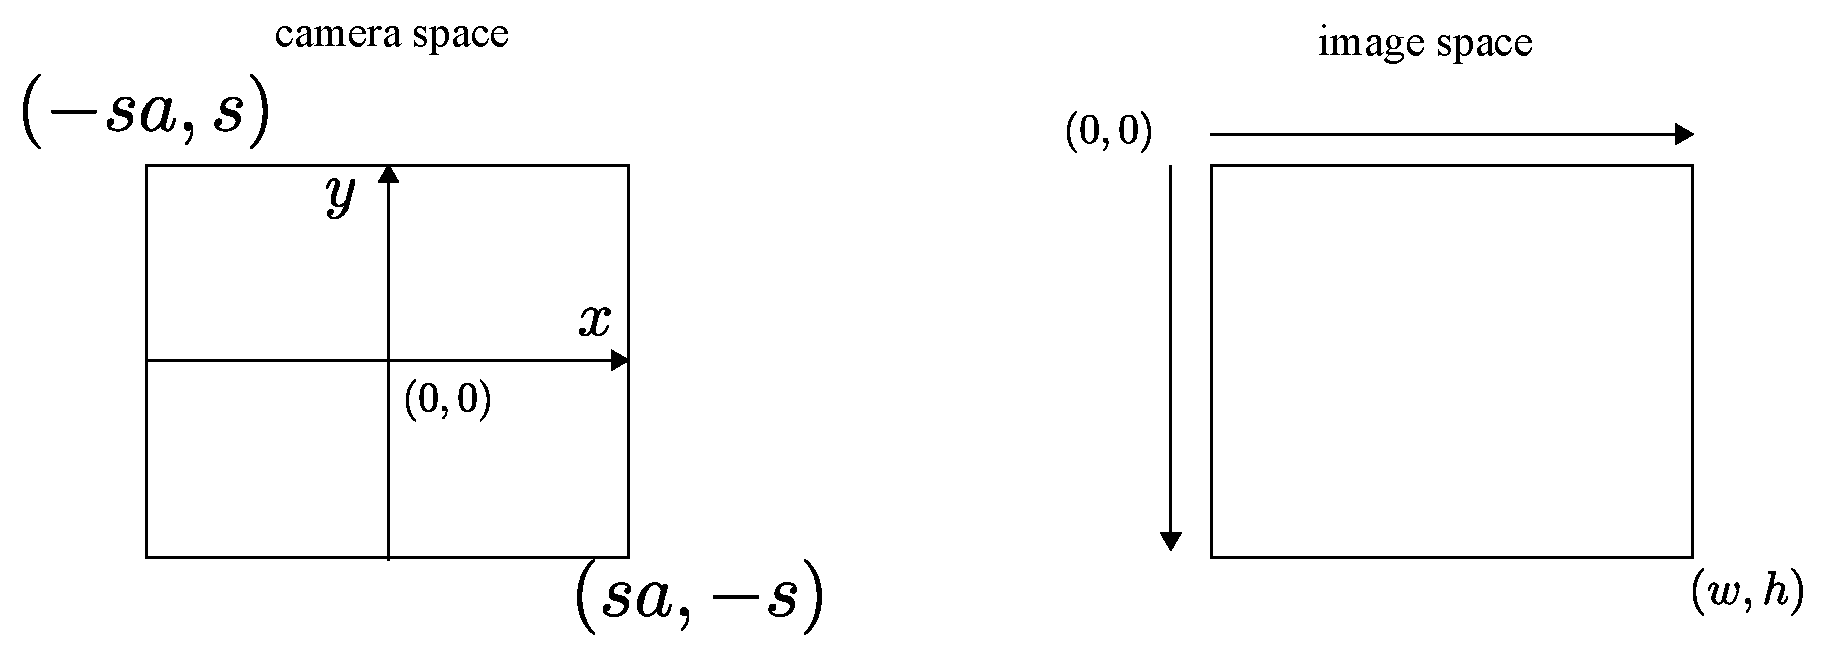
\includegraphics[width=0.9\linewidth]{imgs/camera_vs_image.pdf}
    \caption{The different coordinate systems between our camera space and image space.}
    \label{fig:camera_vs_image}
\end{figure}

There are a few other complications though. Firstly, the point $(x', y')$ is in the (projected) camera space after the projection. We will need to transform it into the screen space. Recall that our screen space has $x$-axis pointing right with $y$-axis pointing down, and the extent is $[0, 0] \times [\text{width}, \text{height}]$. See \cref{fig:camera_vs_image}. So we need to further convert the point $(x', y')$ from the projected camera space to image space. Looking at \cref{fig:camera_vs_image}, we can see that the we need to translate the origin, scale the axes, and flip the $y$ axis. We will give you the formula for the $x$-axis, and you should figure out the $y$-axis formula yourself:
\begin{equation}
x'' = w\frac{x'+sa}{2sa},
\label{eq:camera_to_screen}
\end{equation}
where $w$ is the width of the image.

The second complication is that a triangle vertex can be behind the camera i.e., $z < 0$. In fact, even if $z$ is very close to zero, it can be still problematic: recall that in \cref{eq:projection}, we need to divide by $z$ for the projection. When $z$ is very close to zero, the division can be unstable due to limited floating point precision. Hence, we consider all points such that $z < z_{\text{near}}$ tp be behind the camera. $z_{\text{near}}$ is usually called the \emph{near clipping plane}.

Dealing with triangles with only one or two vertices behind the camera, and the other in front of the camera is tricky: we will need to implement \emph{clipping} (described below as a bonus). Instead, in this homework, we only require you only render the triangles where all three vertices are in front of the near plane. If even one of the vertices of a triangle is behind the near clipping plane, you should reject the triangle and not render it.

\begin{figure}[h]
    \centering
    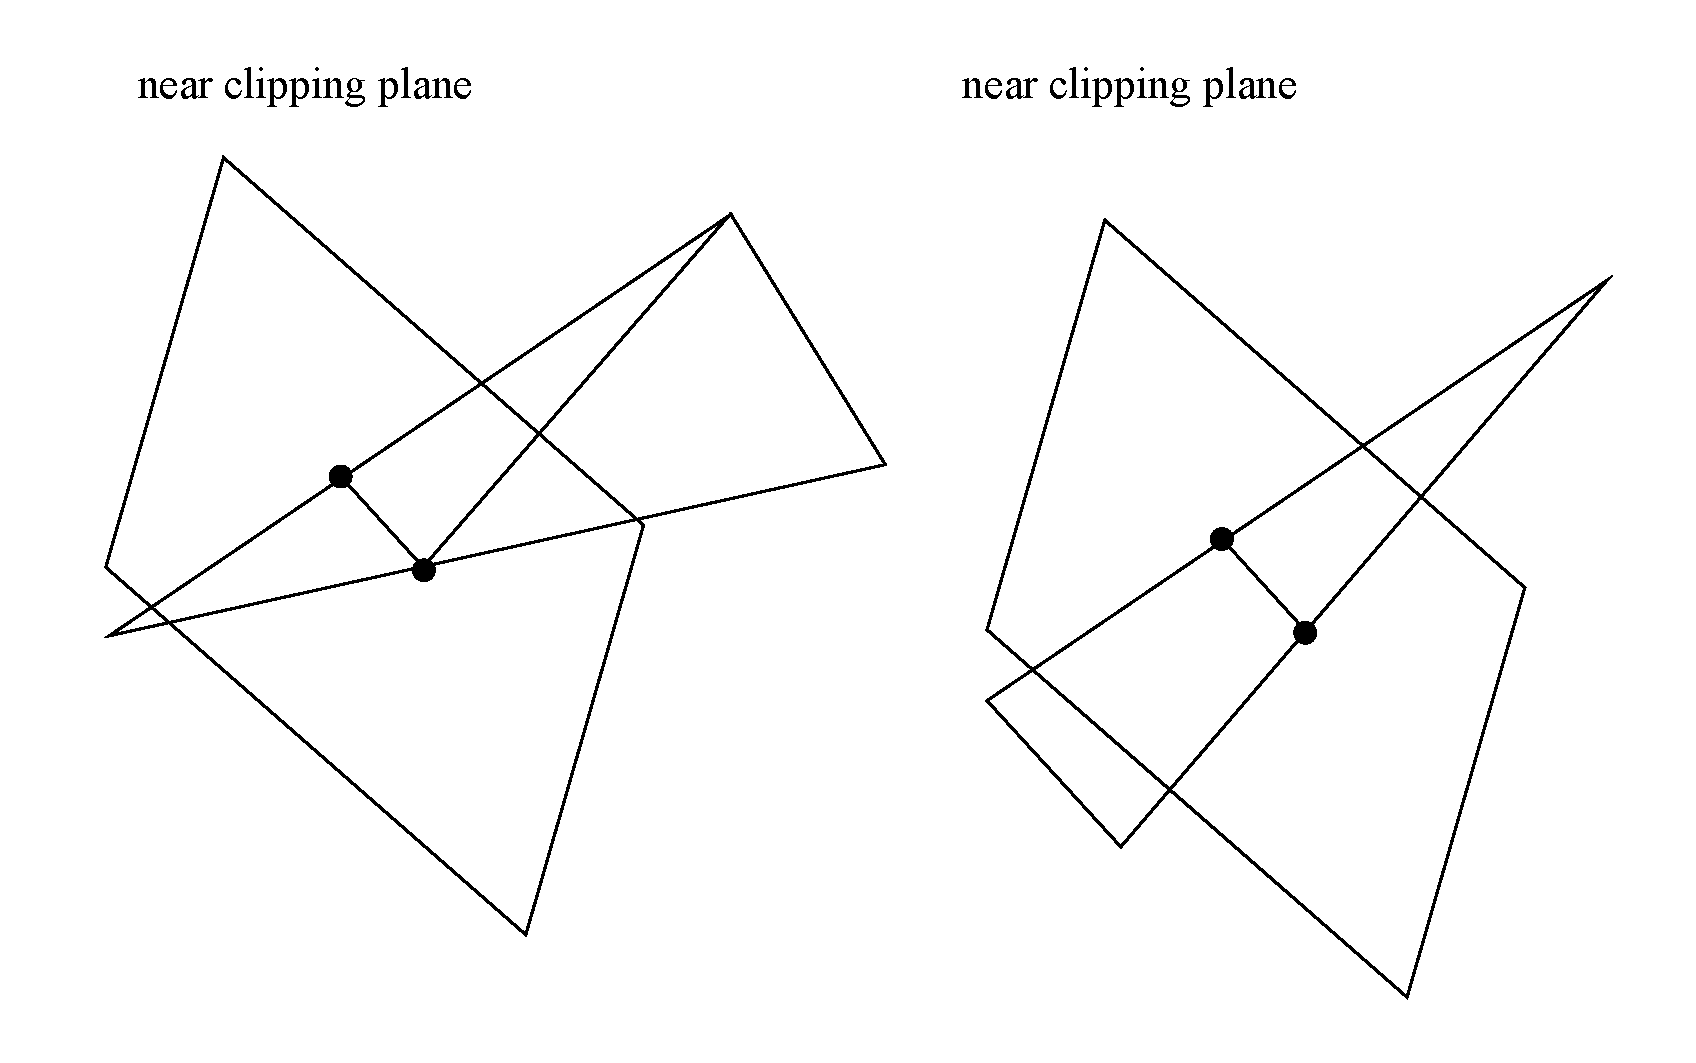
\includegraphics[width=0.7\linewidth]{imgs/triangle_clipping.pdf}
    \caption{If one or two vertices of a triangle is behind the near clipping plane, then (ideally) we would need to clip the triangle. If only one vertex is behind the clipping plane (left), then we need to clip and further split the resulting quadliteral into two triangles. If two vertices are behind the clipping plane (right), the clipped triangle is still a triangle.}
    \label{fig:triangle_clipping}
\end{figure}

Implement your triangle rendering in \lstinline{hw_2_1()} in \lstinline{hw2.cpp}. To test your rendering, use the following command:
\begin{lstlisting}[language=bash]
  ./balboa -hw 2_1 -s 1 -p0 -1 -1 -3 -p1 0 1 -3 -p2 1 -1 -3 -color 0.7 0.3 0.4 -znear 1e-6
\end{lstlisting}

We'll use the same antialiasing scheme we used in Homework 1, i.e., a $4\times4$ supersampling.

We provide our rendering in \cref{fig:hw2_1}.
\begin{figure}[h]
    \centering
    
\includegraphics[width=0.5\linewidth]{imgs/hw_2_1.png}
    \caption{Reference rendering for homework 2.1.}
    \label{fig:hw2_1}
\end{figure}

\paragraph{Bonus: triangle clipping.} In practice, instead of rejecting a triangle if one or two verices are behind the near clipping plane, graphics pipelines would implement triangle clipping (\cref{fig:triangle_clipping}). As a bonus, you will implement the clipping of the triangles and render them correctly even when some vertices are behind the near clipping plane.

\section{Rendering a triangle mesh}

\begin{figure}[h]
    \centering
    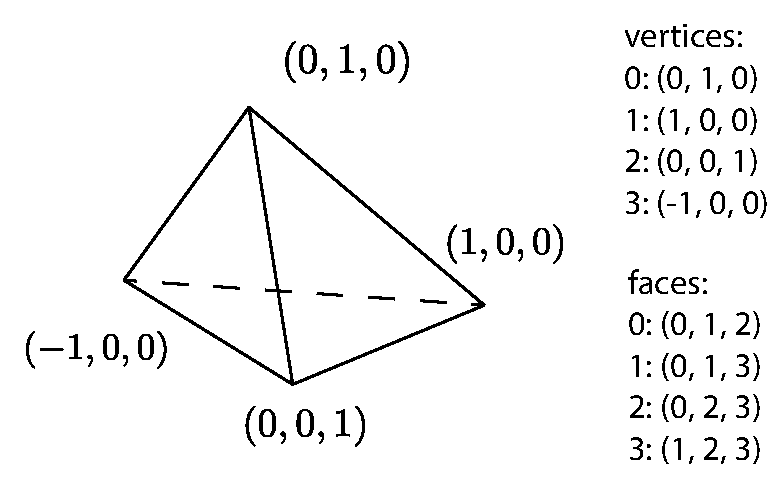
\includegraphics[width=0.7\linewidth]{imgs/triangle_mesh.pdf}
    \caption{A triangle mesh contains a list of vertices (3D positions) and a list of faces (3 integers pointing towards the index of the vertices). The figure shows a case of a triangle mesh with 4 vertices and 4 faces/triangles. The first face represents the triangle on the right side, the second face represents the triangle at the back, the third face represents the triangle on the left, and the last face represents the triangle at the bottom.}
    \label{fig:triangle_mesh}
\end{figure}

Next, we'll extend our previous code to handle more than one triangle. In computer graphics, we often store these triangles in a data structure called ``triangle mesh'' (\cref{fig:triangle_mesh}). Triangle mesh is a more efficient data structure than simply storing a list of triangles since many of the triangles would share vertices in graphics (really? when will it be better and when will it not be better?). To render triangle meshes, you need to go through the face array and loop through all the triangles. 

\begin{figure}[h]
    \centering
    
\includegraphics[width=0.4\linewidth]{imgs/cyclic.pdf}
    
\includegraphics[width=0.4\linewidth]{imgs/interpenetration.pdf}
    \caption{We cannot globally sort all objects into a single order by depth. The objects can form a cyclic order (left) or they can have interpenetration (right).}
    \label{fig:depth_order}
\end{figure}

An important difference, compared to the list of triangles we have in Homework 1, is to determine the depth order between all these triangles. That is, for a point inside a pixel, we need to decide which triangle is the one we actually see. The tricky part is, unlike Homework 1, it is impossible to globally sort the triangles to determine a depth order (\cref{fig:depth_order}).

Therefore, we need to know the depth value of all the triangles overlapping with the point in the pixel. That is, given a image space point inside a projected triangle, we need to \emph{interpolate} from the depth values of the three vertices. This turns out to be slightly involved mathematically (code-wise it's actually just not that much though, my implementation of the depth interpolation takes around 70 lines including lots of comments). 

To explain how to find the desired depth value, we need to explain what are \href{https://en.wikipedia.org/wiki/Barycentric_coordinate_system}{barycentric coordinates}. Any point $\mathbf{p}$ inside a triangle with three vertices $\mathbf{p}_0$, $\mathbf{p}_1$, $\mathbf{p}_2$ can be expressed using linear combination of the three vertices:
\begin{equation}
\mathbf{p} = b_0 \mathbf{p}_0 + b_1 \mathbf{p}_1 + b_2 \mathbf{p}_2,
\end{equation}
where $b_0 + b_1 + b_2 = 1$, $b_0 \geq 0$, $b_1 \geq 0$, and $b_2 \geq 0$. Given a point $\mathbf{p}$, we can compute the \textbf{unique} coefficients using \href{https://en.wikipedia.org/wiki/Cramer%27s_rule}{Cramer's rule}:
\begin{equation}
\begin{aligned}
b_0 &= \frac{\text{area}\left(p, p_1, p_2\right)}{\text{area}\left(p_0, p_1, p_2\right)} \\
b_1 &= \frac{\text{area}\left(p_0, p, p_2\right)}{\text{area}\left(p_0, p_1, p_2\right)} \\
b_2 &= \frac{\text{area}\left(p_0, p_1, p\right)}{\text{area}\left(p_0, p_1, p_2\right)}
\end{aligned}
\label{eq:barycentric_solve}
\end{equation}

To get the area of a triangle, you can use the length of the cross product between two of the edge vectors, which will give you the area of the parallelogram, you can then divide the parallelogram area by two. This works also for 2D triangles, you only need to pretend the 2D triangle is on a 3D plane (e.g., $z=0$).

\begin{figure}[h]
    \centering
    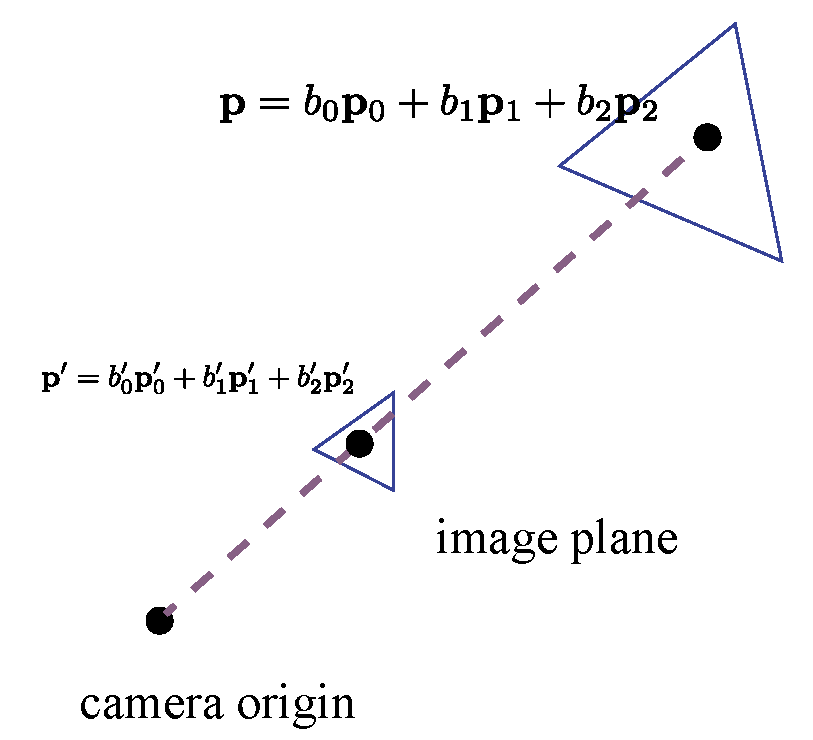
\includegraphics[width=0.5\linewidth]{imgs/perspective_interpolate.pdf}
    \caption{Given a point on image plane $p$', and a triangle with three vertices $\mathbf{p}_0$, $\mathbf{p}_1$, $\mathbf{p}_2$, we want to know the depth, i.e., the $z$ coordinate at the corresponding point $\mathbf{p}$.}
    \label{fig:perspective_interpolate}
\end{figure}

As illustrated in \cref{fig:perspective_interpolate}, our goal is, given an image plane point $\mathbf{p}'$ and a triangle with three vertices $\mathbf{p}_0$, $\mathbf{p}_1$, and $\mathbf{p}_2$, figure out the $z$ coordinate of the corresponding point $\mathbf{p}$. We want to use barycentric coordinates to help us. So we need to figure out what $b_0$, $b_1$, and $b_2$ are, so that we can interpolate the $z$ coordinates from $\mathbf{p}_0$, $\mathbf{p}_1$, and $\mathbf{p}_2$. Unfortunately, we cannot directly use \cref{eq:barycentric_solve}, since we don't know $\mathbf{p}$ (otherwise we would have know the answer already!). 

What we do know are the projected vertices $\mathbf{p}_0'$, $\mathbf{p}_1'$, and $\mathbf{p}_2'$, and our image plane point $\mathbf{p}'$. Furthermore, we know that $p$ projects to $p'$. Given the projected vertices and the image plane point, we can compute the projected barycentric coordinates $b_0'$, $b_1'$, $b_2'$. We want to relate the projected barycentric coordinates with the original ones.

Since $\mathbf{p}$ projects to $\mathbf{p}'$, we know that
\begin{equation}
\begin{aligned}
\mathbf{p}' &= \left(-\frac{\mathbf{p}.x}{\mathbf{p}.z}, -\frac{\mathbf{p}.y}{\mathbf{p}.z}, -1\right) \\
\mathbf{p}' &= -\frac{\mathbf{p}}{\mathbf{p}.z}.
\end{aligned}
\end{equation}

Plugging in $\mathbf{p} = b_0 \mathbf{p}_0 + b_1 \mathbf{p}_1 + b_2 \mathbf{p}_2$ and $\mathbf{p}.z = b_0 \mathbf{p}_0.z + b_1 \mathbf{p}_1.z + b_2 \mathbf{p}_2.z$:
\begin{equation}
\mathbf{p}' = -\frac{b_0 \mathbf{p}_0 + b_1 \mathbf{p}_1 + b_2 \mathbf{p}_2}{b_0 \mathbf{p}_0.z + b_1 \mathbf{p}_1.z + b_2 \mathbf{p}_2.z}.
\end{equation}

Next, we know that $\mathbf{p}_0$ projects to $\mathbf{p}_0'$, $\mathbf{p}_1$ projects to $\mathbf{p}_1'$, and $\mathbf{p}_2$ projects to $\mathbf{p}_2'$:
\begin{equation}
\begin{aligned}
-\left(\mathbf{p}_0.z\right) \left(\mathbf{p}_0'\right) &= \mathbf{p}_0 \\
-\left(\mathbf{p}_1.z\right) \left(\mathbf{p}_1'\right) &= \mathbf{p}_1 \\
-\left(\mathbf{p}_2.z\right) \left(\mathbf{p}_2'\right) &= \mathbf{p}_2.
\end{aligned}
\end{equation}

Plugging in, we get
\begin{equation}
\mathbf{p}' = \frac{b_0 \left(\mathbf{p}_0.z\right) \mathbf{p}_0' + b_1 \left(\mathbf{p}_1.z\right) \mathbf{p}_1' + b_2 \left(\mathbf{p}_2.z\right) \mathbf{p}_2'}{b_0 \mathbf{p}_0.z + b_1 \mathbf{p}_1.z + b_2 \mathbf{p}_2.z}.
\end{equation}

Compare the above with:
\begin{equation}
\mathbf{p}' = b_0' \mathbf{p}_0' + b_1' \mathbf{p}_1' + b_2' \mathbf{p}_2',
\end{equation}
using the uniqueness of barycentric coordinates, we have:
\begin{equation}
\begin{aligned}
b_0' &= \frac{b_0 \mathbf{p}_0.z}{b_0 \mathbf{p}_0.z + b_1 \mathbf{p}_1.z + b_2 \mathbf{p}_2.z} \\
b_1' &= \frac{b_1 \mathbf{p}_1.z}{b_0 \mathbf{p}_0.z + b_1 \mathbf{p}_1.z + b_2 \mathbf{p}_2.z} \\
b_2' &= \frac{b_2 \mathbf{p}_2.z}{b_0 \mathbf{p}_0.z + b_1 \mathbf{p}_1.z + b_2 \mathbf{p}_2.z}.
\end{aligned}
\label{eq:projected_barycentric}
\end{equation}

We are almost there: we now want to express $b_0$, $b_1$, and $b_2$ using $b_0'$, $b_1'$, and $b_2'$. Let $B = b_0 \mathbf{p}_0.z + b_1 \mathbf{p}_1.z + b_2 \mathbf{p}_2.z$, we have:
\begin{equation}
\begin{aligned}
b_0 &= \frac{b_0' B}{\mathbf{p}_0.z} \\
b_1 &= \frac{b_1' B}{\mathbf{p}_1.z} \\
b_2 &= \frac{b_2' B}{\mathbf{p}_2.z}
\end{aligned}
\end{equation}

Furthermore, we know that $b_0 + b_1 + b_2 = 1$, so:
\begin{equation}
B = \frac{1}{\frac{b_0'}{\mathbf{p}_0.z} + \frac{b_1'}{\mathbf{p}_1.z} + \frac{b_2'}{\mathbf{p}_2.z}}.
\end{equation}

Rewriting \cref{eq:projected_barycentric} using the equation above, we have:
\begin{equation}
\begin{aligned}
\frac{\frac{b_0'}{\mathbf{p}_0.z}}{\frac{b_0'}{\mathbf{p}_0.z} + \frac{b_1'}{\mathbf{p}_1.z} + \frac{b_2'}{\mathbf{p}_2.z}} &= b_0 \\
\frac{\frac{b_1'}{\mathbf{p}_1.z}}{\frac{b_0'}{\mathbf{p}_0.z} + \frac{b_1'}{\mathbf{p}_1.z} + \frac{b_2'}{\mathbf{p}_2.z}} &= b_1 \\
\frac{\frac{b_2'}{\mathbf{p}_1.z}}{\frac{b_0'}{\mathbf{p}_0.z} + \frac{b_1'}{\mathbf{p}_1.z} + \frac{b_2'}{\mathbf{p}_2.z}} &= b_2
\end{aligned}.
\label{eq:inverse_depth_weighting}
\end{equation}
The equation above has an intuitive meaning: \textbf{the original barycentric coordinates can be obtained by the projected barycentric coordinate weighted by inverse depth}. We will use these equations again later in the homework.

Having the barycentric coordinates, we can finally get the desired depth:
\begin{equation}
\mathbf{p}.z = b_0 \mathbf{p}_0.z + b_1 \mathbf{p}_1.z + b_2 \mathbf{p}_2.z.
\label{eq:interpolated_depth}
\end{equation}

To recap: given an image plane point and a triangle, we first convert it from screen space to camera space (using the inverse of \cref{eq:camera_to_screen}, recall \cref{fig:camera_vs_image}). Then, we compute the projected barycentric coordinates $b_0'$, $b_1'$, and $b_2'$ using \cref{eq:barycentric_solve}. Using the projected barycentric coordinates and the depth at the three vertices, we convert them to the original barycentric coordinates using \cref{eq:inverse_depth_weighting}. Finally, we obtain the depth using \cref{eq:interpolated_depth} and use the depth to pick the triangle that is the closest to the pixel sample, but in front of the clipping plane.

One final detail, remember we discussed two variants for rendering multiple objects in a scene? The depth testing makes the two variants differ more. For the \emph{ray tracing} style (i.e., for each pixel, check all triangles), you need to maintain a minimal $z$ value when traversing all the triangles. For the \emph{rasterization} style (i.e., for each triangle, check all pixels), you need to maintain a whole image of $z$ values, and this is usually called the \emph{Z-buffer}. 
\begin{lstlisting}[language=Python]
# For each pixel, check all triangles
for each pixel:
    z_min = infinity
    for each triangle:
        # check if the pixel center hits the triangle
        # overwrite color and z_min if the triangle is closer

# For each triangle, check all pixels
Z_buffer = Image(w, h)
for each triangle:
    # project the triangle
    for each pixel:
        # check if the pixel center hits the triangle
        # overwrite color and Z_buffer[pixel] if the triangle is closer
\end{lstlisting}
We will discuss the pros and cons of the two approaches in depth in the lectures.

Now you should be ready to implement the rendering of a triangle mesh! In this part, to specify the color of the triangles, in our triangle mesh, we further store a color per triangle. 

Our \lstinline{TriangleMesh} data structure looks like this:
\begin{lstlisting}[language=C++]
struct TriangleMesh {
    std::vector<Vector3> vertices; // 3D positions of the vertices
    std::vector<Vector3i> faces; // indices of the triangles
    std::vector<Vector3> face_colors; // per-face color of the mesh, only used in HW 2.2
    std::vector<Vector3> vertex_colors; // per-vertex color of the mesh, used in HW 2.3 and later
};
\end{lstlisting}
\lstinline{faces} and \lstinline{face_colors} will always be the same length.

Go implement your triangle mesh rendering code in \lstinline{hw_2_2}. To test your implementation, use the command
\begin{lstlisting}[language=bash]
  ./balboa -hw 2_2 -s 1 -znear 1e-6 -scene_id 0
\end{lstlisting}

Our rendering for \lstinline{scene_id 0} is in \cref{fig:hw2_2}.
\begin{figure}[h]
    \centering
    
\includegraphics[width=0.5\linewidth]{imgs/hw_2_2.png}
    \caption{Reference rendering for homework 2.2.}
    \label{fig:hw2_2}
\end{figure}

\section{Perspective-corrected interpolation}

So far, we have been rendering constant color triangles. It's time to make things more colorful. Instead of specifying \emph{face colors}, we'll specify \emph{vertex colors}, and interpolate them using barycentric coordinates.

It might be tempting to use the projected barycentric coordinates ($b_0', b_1'$ and $b_2'$) to interpolate the vertex colors, but this is incorrect: our triangle would be changing color based on the vertex depth if we do this (try it!). Instead, we want to interpolate using the original barycentric coordinates $b_0$, $b_1$, and $b_2$. Fortunately, we already know how to get them using \cref{eq:inverse_depth_weighting}! After computing the original barycentric coordinates, we'll just interpolate the vertex colors $C_0$, $C_1$, $C_2$ defined at the triangle vertices:
\begin{equation}
C = b_0 C_0 + b_1 C_1 + b_2 C_2.
\end{equation}
This is what people mean if they say they are doing \emph{perspective-corrected interpolation} in a renderer.

That's all you need to know to implement vertex color rendering! (I hope it's easier than the previous two.) Go and implement it in \lstinline{hw_2_3}.

\section{3D transformation}

\section{Design your own scenes}

%\bibliographystyle{plain}
%\bibliography{refs}

\end{document}
